% ---------------------------------------------------------------------------
%  DIY presentation -- 15 + 5 minutes
%  Aryan Bandyopadhyay (2411014), PHY341/745
%
%  Compile:  pdflatex slides.tex     (figures in ../figures/)
%  A no-LaTeX alternative with the same content: deck.html
% ---------------------------------------------------------------------------
\documentclass[aspectratio=169,10pt]{beamer}

\usepackage[T1]{fontenc}
\usepackage{lmodern}
\usepackage{amsmath,amssymb}
\usepackage{graphicx}
\usepackage{booktabs}

\graphicspath{{../figures/}}

\definecolor{ink}{HTML}{1B1B1B}
\definecolor{accent}{HTML}{1F4E79}
\definecolor{accent2}{HTML}{A8322D}
\definecolor{faint}{HTML}{6B6B6B}

\setbeamercolor{normal text}{fg=ink}
\setbeamercolor{structure}{fg=accent}
\setbeamercolor{frametitle}{fg=accent}
\setbeamercolor{alerted text}{fg=accent2}
\setbeamertemplate{navigation symbols}{}
\setbeamertemplate{itemize items}[circle]
\setbeamerfont{frametitle}{size=\large,series=\bfseries}
\setbeamerfont{footline}{size=\scriptsize}
\setbeamertemplate{footline}{%
  \hfill\usebeamerfont{footline}\color{faint}%
  Burgers / 1-D Navier--Stokes \quad\textbar\quad Aryan Bandyopadhyay (2411014)
  \quad\textbar\quad \insertframenumber\,/\,\inserttotalframenumber\hspace{4mm}\vspace{2mm}}

\newcommand{\hl}[1]{\textcolor{accent2}{\textbf{#1}}}

\title{\textbf{Shock waves in a one-dimensional fluid}}
\subtitle{How much of what you see is the grid?}
\author{Aryan Bandyopadhyay \, (2411014)}
\institute{PHY341/745 Physics Computer Lab \,--\, DIY project \\ NISER Bhubaneswar}
\date{}

\begin{document}

% 1 -------------------------------------------------------------------
\begin{frame}
  \titlepage
  \note{30 s. Do not read the title. Say: "I solved one equation five ways,
  and the five answers disagree. This talk is about which of them to believe."}
\end{frame}

% 2 -------------------------------------------------------------------
\begin{frame}{One equation}
  \begin{columns}[T]
    \begin{column}{0.52\textwidth}
      \[ u_t + u\,u_x = \nu\,u_{xx} \]
      \vspace{-2mm}
      \begin{itemize}
        \item nonlinearity steepens the wave
        \item viscosity smooths it
        \item the balance is a \hl{shock}
      \end{itemize}
      \vspace{2mm}
      \small
      In one dimension, incompressibility forces $\partial_xu=0$: advection and
      the pressure gradient both vanish. Dropping only the pressure gradient
      leaves this --- the \hl{1-D Navier--Stokes} equation.
    \end{column}
    \begin{column}{0.46\textwidth}
      \centering
      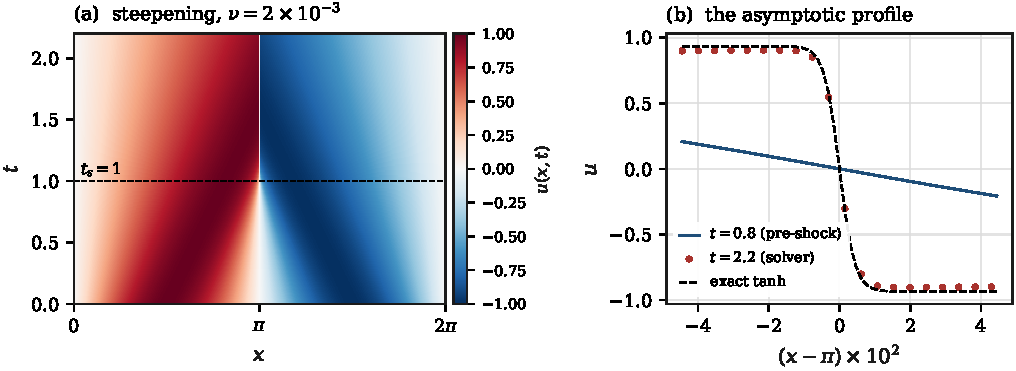
\includegraphics[width=\textwidth]{fig02_shock_formation.pdf}\\
      \scriptsize the whole talk, in one picture
    \end{column}
  \end{columns}
  \note{1 min. This is the only physics in the talk. Say explicitly that the
  course does not require the physics, so you will spend the time on numerics.}
\end{frame}

% 3 -------------------------------------------------------------------
\begin{frame}{The only theory needed}
  \begin{columns}[T]
    \begin{column}{0.5\textwidth}
      \textbf{When does it break?}\\[1mm]
      Characteristics $x=\xi+u_0(\xi)t$ cross at
      \[ t_s = -\frac{1}{\min u_0'} = 1 \quad (u_0=\sin x). \]
      After that: a shock.

      \vspace{4mm}
      \textbf{How thick is it?}
      \[ \delta = \frac{4\nu}{U}, \qquad
         u = -U\tanh\!\frac{U(x-x_0)}{2\nu}. \]
    \end{column}
    \begin{column}{0.47\textwidth}
      \small
      Everything in this talk is measured against one of these two formulas,
      or against
      \[ E(k)\propto k^{-2}, \qquad \zeta_p=\min(p,1). \]
      \vspace{1mm}
      \color{faint}
      Four predictions, no free parameters. That is what makes the \emph{numerics}
      measurable rather than decorative.
    \end{column}
  \end{columns}
  \note{1 min. Derive t_s on the board if asked; it takes three lines. The tanh
  profile is the exact steady solution --- verify it by substitution.}
\end{frame}

% 4 -------------------------------------------------------------------
\begin{frame}{Five solvers, three diagnostics}
  \begin{columns}[T]
    \begin{column}{0.55\textwidth}
      \small
      \begin{tabular}{@{}ll@{}}
        \toprule
        scheme & order \\
        \midrule
        upwind & 1 \\
        Lax--Wendroff & 2 \\
        FTCS & 2 (unstable) \\
        Crank--Nicolson + Heun & 2 \\
        spectral, Strang + RK4 & exponential \\
        \bottomrule
      \end{tabular}
      \vspace{3mm}

      All written for this project. NumPy only for arrays: no \texttt{np.fft},
      no \texttt{scipy}. The FFT is radix-2, checked against a naive DFT to
      $10^{-15}$.
    \end{column}
    \begin{column}{0.42\textwidth}
      \small
      \textbf{Diagnostics}\\
      $\delta$ = jump / max slope\\
      $E(k)$ from a from-scratch FFT\\
      $S_p(r)$ = moment of increments\\[2mm]
      \textbf{Reference}\\
      exact Cole--Hopf solution, grid-independent to $10^{-12}$
    \end{column}
  \end{columns}
  \note{1 min. Emphasise: the reference is analytic, not "a very fine run".
  That is the methodological core.}
\end{frame}

% 5 -------------------------------------------------------------------
\begin{frame}{Result 1 --- are the solvers right?}
  \centering
  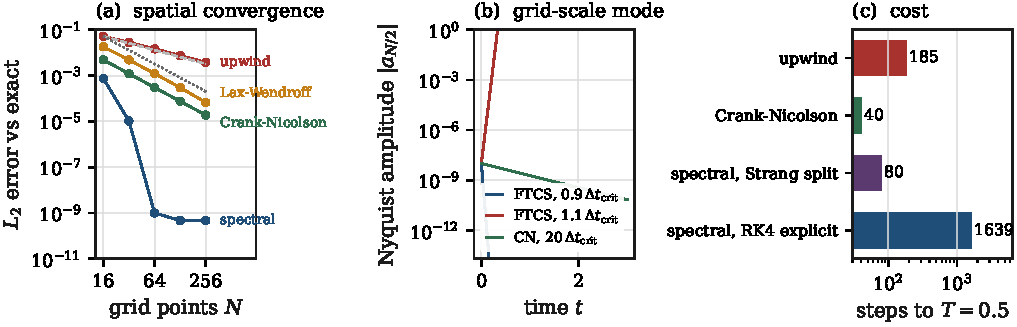
\includegraphics[width=\textwidth]{fig01_validation.pdf}
  \vspace{-2mm}
  \small
  measured orders \hl{0.94, 2.02, 2.00}, spectral $7.5\times10^{-4}\!\to\!10^{-9}$;
  measured growth rates match von Neumann to \hl{0.3\%}.
  \note{3 min. Panel (a): the spectral curve is exponential until the Strang
  floor --- explain why. Panel (b): the scheme is unstable exactly where theory
  says. Panel (c): the cost of being explicit.}
\end{frame}

% 6 -------------------------------------------------------------------
\begin{frame}{Result 2 --- breaking, and what is left behind}
  \centering
  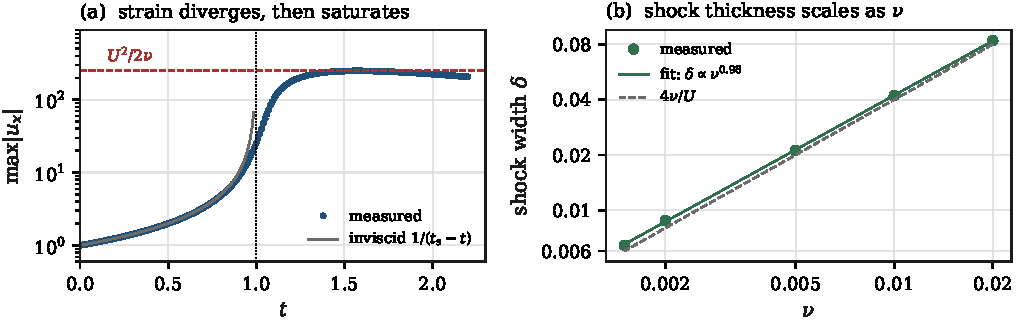
\includegraphics[width=0.92\textwidth]{fig03_shock_scaling.pdf}
  \vspace{-2mm}
  \small
  strain $=\frac{1}{t_s-t}$ to 0.5\%, saturating at \hl{$247.5$ vs $250$};
  $\delta\propto\nu^{\,0.985}$, prefactor 5--10\% above $4\nu/U$.
  \note{2 min. Numbers first: 1.249 vs 1.250. Then say where the 5-10% comes
  from --- finite amplitude of a decaying sawtooth. Honesty here buys credit.}
\end{frame}

% 7 -------------------------------------------------------------------
\begin{frame}{Result 3 --- the spectrum has a movable end}
  \centering
  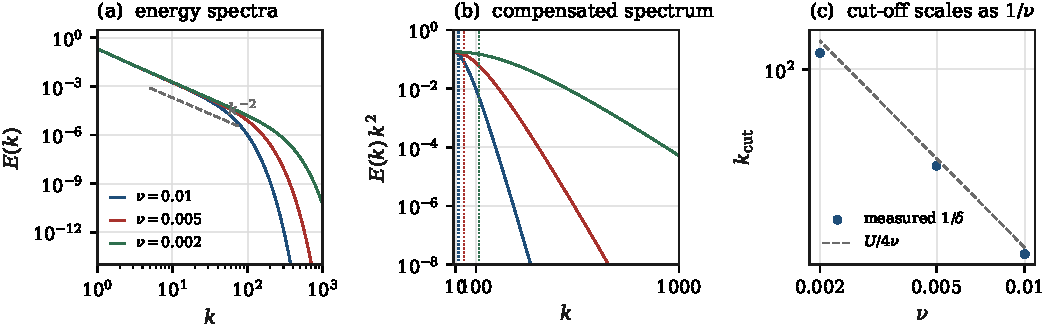
\includegraphics[width=\textwidth]{fig04_spectra.pdf}
  \vspace{-2mm}
  \small
  $E(k)\propto k^{-2.030\pm0.001}$ for every $\nu$; the cut-off
  $k_{\rm cut}\propto\nu^{-0.971}$.
  \note{2 min. The punchline sentence: viscosity does not change the shape of
  the spectrum, only where it ends.}
\end{frame}

% 8 -------------------------------------------------------------------
\begin{frame}{Result 4 --- many shocks: one exponent}
  \centering
  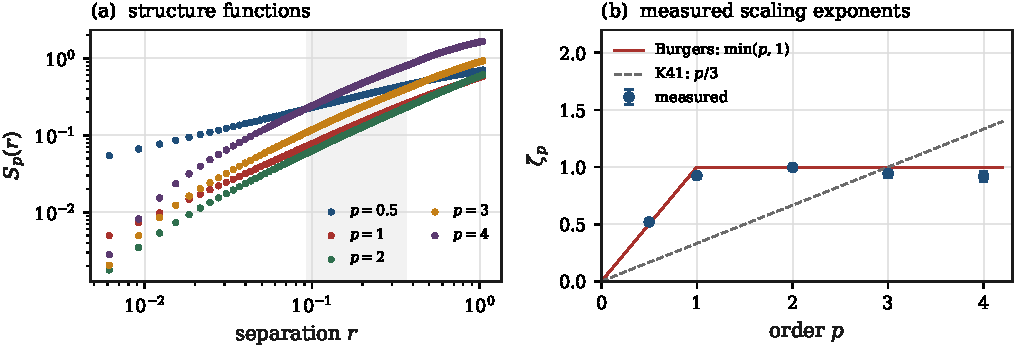
\includegraphics[width=0.95\textwidth]{fig05_structure_functions.pdf}
  \vspace{-2mm}
  \small
  $\zeta_p = 0.52,\ 0.92,\ 1.00,\ 0.94,\ 0.92$ \ vs \ $\min(p,1)$ \ and \ $p/3$:
  a factor of three apart at $p=4$, error bar $5\%$.
  \note{2 min. This is the most impressive-looking result; make sure you can
  state why p>1 all give the same exponent (any moment is dominated by the
  same discontinuities).}
\end{frame}

% 9 -------------------------------------------------------------------
\begin{frame}{Result 5 --- how much of the viscosity is the grid?}
  \centering
  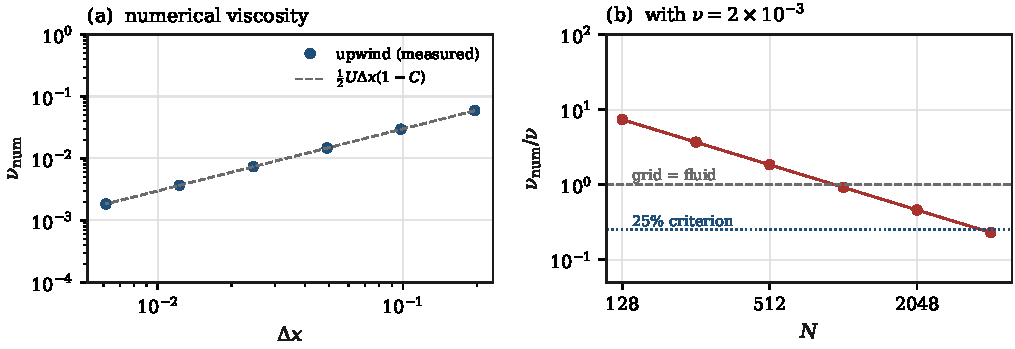
\includegraphics[width=\textwidth]{fig06_grid_viscosity.pdf}
  \vspace{-2mm}
  \small
  $\nu_{\rm num}=\frac12U\Delta x(1-C)$ verified to \hl{1\%} over five decades;
  at $N=256$, \hl{$\nu_{\rm num}=3.7\nu$}.
  \note{2.5 min. The point of the whole project: the grid's viscosity is a
  computable quantity, not a nuisance. End with the criterion
  dx < 0.2 delta.}
\end{frame}

% 10 ------------------------------------------------------------------
\begin{frame}{What I take away}
  \begin{itemize}
    \item Convergence \emph{order} does not predict shock \emph{quality}:
          all four schemes have known orders and disagree qualitatively
          (smeared vs ringed).
    \item Integral quantities are robust; local ones are not. The $k^{-2}$
          slope survives a $10^3$ change in $\nu$; the shock thickness does not.
    \item Numerical dissipation is measurable, has a formula, and should be
          computed rather than hoped away.
  \end{itemize}
  \vspace{3mm}
  \begin{block}{Practical criterion}
    \centering
    resolve the shock, not the wavelength: $\Delta x \lesssim 0.2\,\delta$
    \;\,($\gtrsim 5$ points per shock).
  \end{block}
  \note{1.5 min. Leave time: the professor will ask "how do you know the
  reference is right?" --- answer with the residual test and the band-limited
  interpolation story.}
\end{frame}

% 11 ------------------------------------------------------------------
\begin{frame}{Limitations, and what I would do next}
  \begin{columns}[T]
    \begin{column}{0.48\textwidth}
      \textbf{Limitations}
      \begin{itemize}
        \item inertial range only $\approx1.5$ decades
        \item statistics taken at one time, not stationary
        \item one equation, no vortex stretching (absent in 1-D)
      \end{itemize}
    \end{column}
    \begin{column}{0.48\textwidth}
      \textbf{Next}
      \begin{itemize}
        \item forced, statistically stationary run
        \item WENO/TVD scheme, same $\zeta_p$ test
        \item extension to 2-D
      \end{itemize}
    \end{column}
  \end{columns}
  \note{1 min. Naming your own limitations before they are pointed out is the
  cheapest credibility in a viva.}
\end{frame}

% 12 ------------------------------------------------------------------
\begin{frame}{References}
  \small
  \begin{enumerate}
    \item J. M. Burgers, \emph{A mathematical model illustrating the theory of
          turbulence}, Adv. Appl. Mech. \textbf{1}, 171 (1948).
    \item J. Bec and K. Khanin, \emph{Burgers turbulence},
          Phys. Rep. \textbf{447}, 1 (2007).
    \item G. B. Whitham, \emph{Linear and Nonlinear Waves} (Wiley, 1974),
          ch.~2--4.
    \item R. J. LeVeque, \emph{Finite Volume Methods for Hyperbolic Problems}
          (CUP, 2002), ch.~4, 6.
    \item J. P. Boyd, \emph{Chebyshev and Fourier Spectral Methods}
          (Dover, 2001), ch.~2.
    \item J. D. Cole, \emph{On a quasi-linear parabolic equation occurring in
          aerodynamics}, Quart. Appl. Math. \textbf{9}, 225 (1951).
  \end{enumerate}
  \vspace{6mm}
  \centering
  \hl{Code, figures and every number:}\\[1mm]
  \texttt{github.com/Aryans-lab/Computational\_Physics\_Lab/}\\
  \texttt{project\_burgulence/}
\end{frame}

\end{document}
